\section{\uppercase{Deconstruction App}}
\label{sec:application}

\noindent
A deconstruction oriented to the maximum reuse of materials must be supported by a \emph{workflow} that guides the user towards estimating the costs of the process. The aim is the determination of  \emph{building demolition costs}, depending also on transportation  and disposal of materials.

\subsection{Workflow}

\paragraph{Project definition} 

The first phase of the modeling process is a gross description of the building, in order to provide basic clues for a correct attribution of the semantic attributes.
In particular, we ask for: the apparent age, the style of construction, the historic use register, and the geolocation.
The estimated age and the style of construction are used to determine the needed data about the used materials; the record of use destinations allows you to to reconstruct the hazard notes of the items to be disposed of; geolocation finally allows to find out the recycling facilities closest to the site.

\paragraph{Building modeling} 

The user describes the construction using some predefined classes of elements, either instancing some  predefined parametric plugins or though wire-frame input of 2D layouts. 
First is defined the building skeleton (backbone), i.e.~the set of beams and columns.
On its horizontal sections, the user specifies the exterior and interior walls (vertical enclosure and partitions), on which the fixtures are positioned (horizontal communications).
Ceilings and floors (horizontal partitions) are instead automatically generated from the topology (1-boundary) of the 2-skeleton (set of 2-cells) of the floors.
Finally, various elements such as stairs, elevators (vertical communications), foundations and roofs (horizontal enclosures) are placed, using ad-hoc templates interactively provided by Metior's plugin server, for appropriate sizing and part dimensioning.

\paragraph{Semantic annotations} 

At this stage the previously inserted elements are annotated semantically  by means of references to database of materials, including densities. The annotation may consists of one or more materials, including percentages.
For disposal control imposed by regulations, the user should assign one / more CER codes and degrees of dangerousness (see Section~\ref{sec:CER}).
In this stage it is also assigned a pair of links that refer to the time schedule for disposal of  building components.

\begin{figure}[!h]
  \centering
  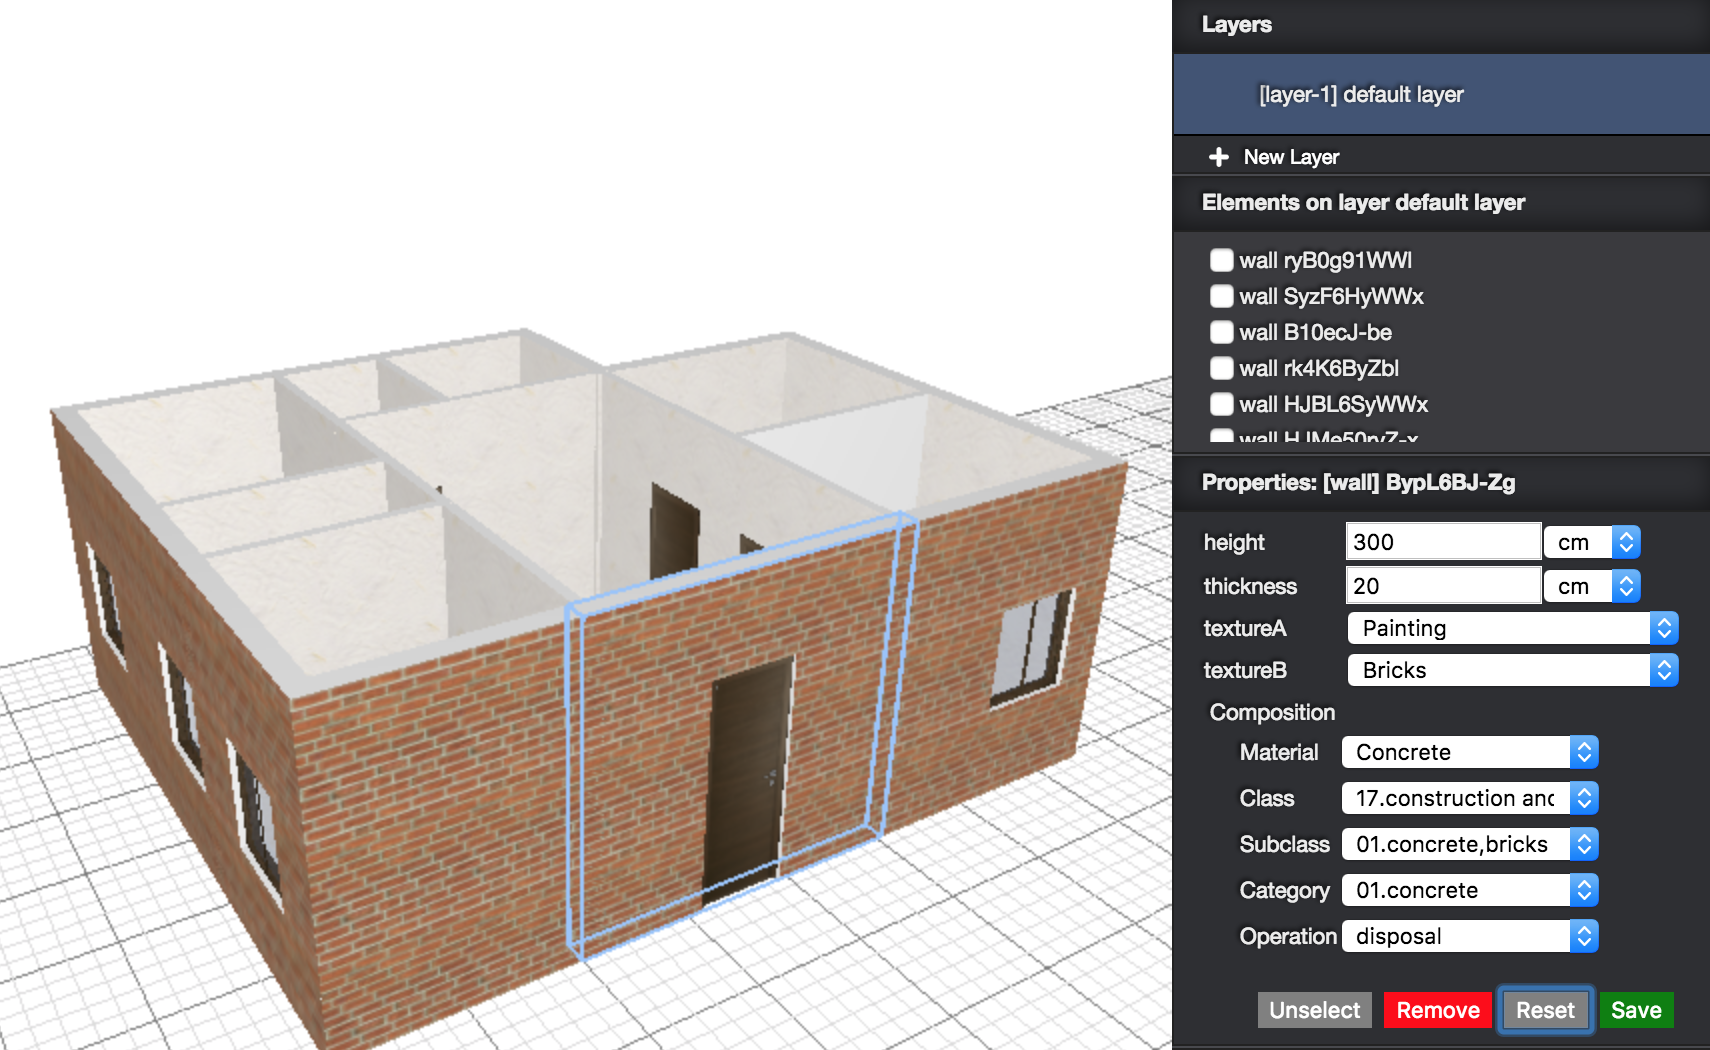
\includegraphics[width=1\linewidth]{images/3d-sel}
  \caption{Graphical interface for semantics annotation of a modeled object}
  \label{fig:semantics}
\end{figure}

\paragraph{Augmented reality visualization} 

After modeling and attribution of semantics to components, the quantity surveyer can validate the entire model by spatial merging into a 3D point cloud (see Figure~\ref{fig:augmented}) previously obtained by using flying drones for the exterior, or 3D laser scanners for the interior. In this way one can assess the adhesion of the modeled building structure to reality, possibly retracing to some previous step if the result is still not satisfactory.

\begin{figure}[htbp] %  figure placement: here, top, bottom, or page
   \centering
   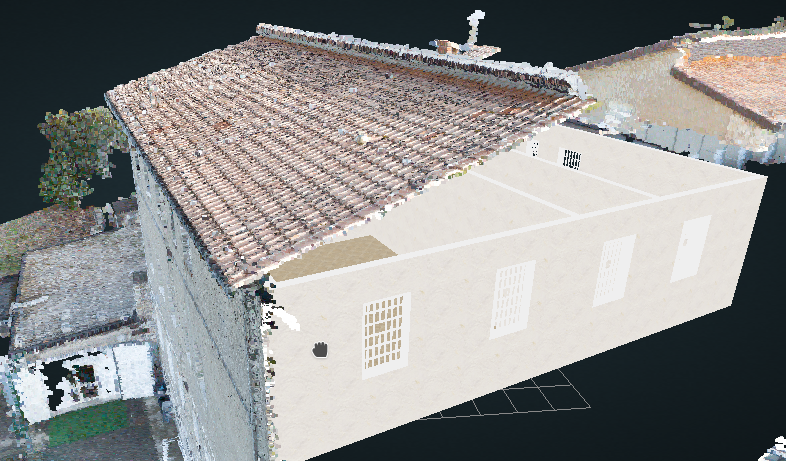
\includegraphics[width=1\linewidth]{images/augmented}
   \caption{A model inside a point cloud}
   \label{fig:augmented}
\end{figure}

\subsection{Process output}

\noindent 
Once the work is done and the model geometry is validated, the application provides a final report.
In particular, the final report will allows the quantity surveyer and/or the other professionals involved in the deconstruction design team, to determine whether the decision taken is convenient both economically and/or environmentally.

The final report consists of four documents.
(i)~\emph{An estimate of volumes and weights of materials}, computed by appropriate integration calculations, based on the geometry of components and annotations defined on them.
(ii)~\emph{An estimate of demolition costs}, including disposal and recovery.
Starting from volumes and densities of materials, and from CER codes and hence the mode of disposal, it is estimated the cost of the contribution to landfills.
(iii)~\emph{The transportation costs} to move the materials to the closest landfills, taking into account the geographical position of the building, and by calculating the most convenient road routes.
(iv)~\emph{An estimate of the expected time} for the complete demolition of the building, located on a Gantt chart. A PERT program, automatically generated while annotating semantically the components of the building, is used for this purpose.

\noindent